\chapter{Architettura del prodotto}\label{ArchitetturaDelProdotto}

\section{Descrizione generale}
In fase di progettazione, il gruppo \textit{Jawa Druids} ha deciso di suddividere la modellazione architetturale di \textit{Gathering-Detection-Platform} in tre distinti moduli, tutti indipendenti tra loro.
Il primo modulo si occupa solamente di leggere, tramite file JSON$_G$, tutte le webcam disponibili per poi effettuare il riconoscimento persone tramite i frame scaricati. Successivamente i dati estrapolati verranno invitati al database.
Il secondo modulo, il machine-learning$_G$, si occupa di recuperare questi dati dal database per lavorarli producendo predizioni per le ore future.
Infine il terzo modulo, la web-app$_G$ vera e propria, si occuperà di rappresentare graficamente i dati all'interno del database mediante una heat-map$_G$ e farli visualizzare all'utente.

\section{Architettura acquisizione}\label{ArchitetturaDelProdottoAcquisition}
L'architettura riguardante il modulo di acquisizione, ovvero il primo modulo del software, è molto semplice ed intuitiva.
Non vi è alcuna classe e si basa su una programmazione procedurale.
Nel \textit{detect.py}, ovvero lo script principale del modulo, vengono richiamate le funzioni, in maniera sequenziale, per scaricare e manipolare i dati delle webcam.
La scelta dell'utilizzo di un paradigma procedurale risiede nel fatto che la creazione di oggetti e il loro utilizzo risultavano, nell'insieme, più complicati mentre chiamando delle semplici funzioni esterne il programma risultava più leggibile ed efficiente.
Gli unici oggetti presenti in \textit{detect.py} sono quelli di tipo \textit{data}, necessari per la giusta esecuzione dello script.
Di seguito vengono riportati i diagrammi relativi all'\textit{attività} e di \textit{package}.
%Inserire
%Grafici

\subsection{Diagramma dei package dell'acquisizione}\label{DiagrammaDeiPackageAcquisition}
%Inserire PACKAGE
\begin{center}
	\begin{figure}[H]
		\centering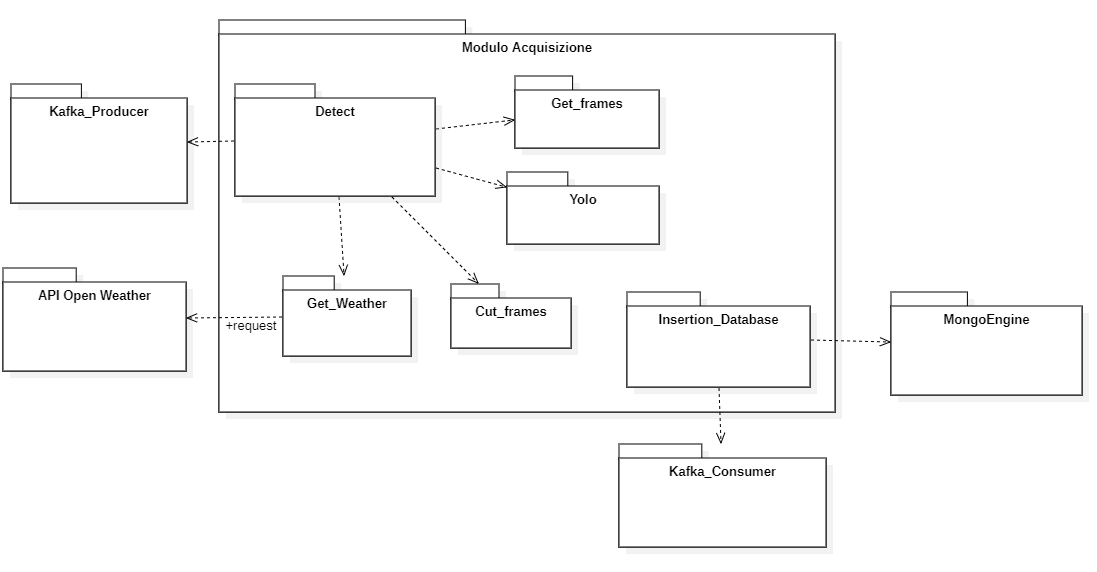
\includegraphics[scale=0.65]{../immagini/diag_PB/diag_pack_acqui.png}
		\caption{Diagramma dei package del modulo acquisition}
	\end{figure}
\end{center}

\subsection{Diagramma di attività}
\begin{center}
	\begin{figure}[H]
		\centering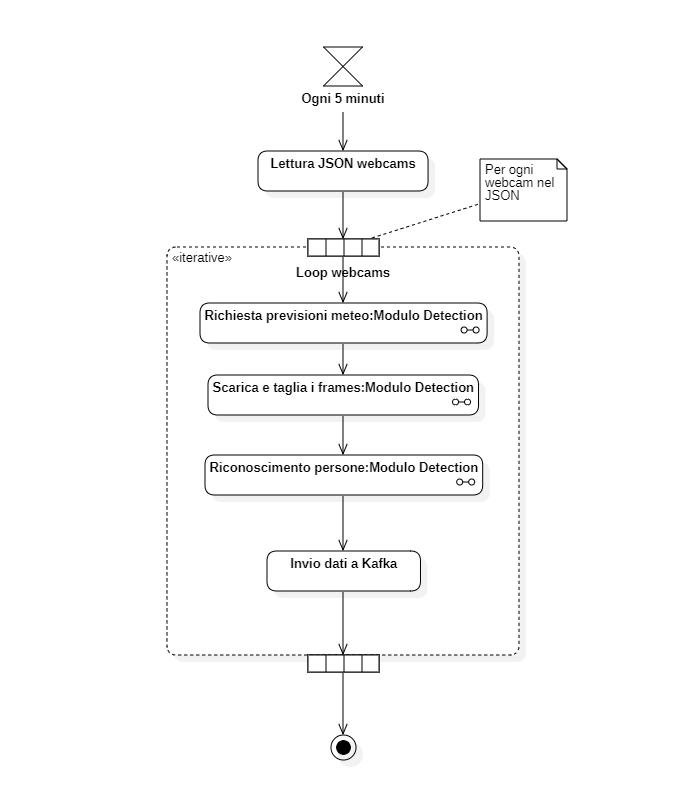
\includegraphics[scale=0.65]
    {../immagini/diag_PB/detection.png}
		\caption{Diagramma di attività del modulo Acquisition}
	\end{figure}
\end{center}

\subsubsection{Diagramma di sotto attività di richiesta previsioni meteo}\label{DiagrammaSottoAttivitaRichiestaPrevisioniMeteo}
\begin{center}
	\begin{figure}[H]
		\centering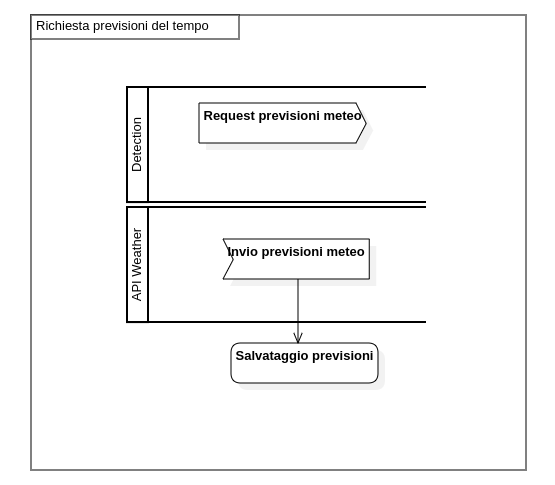
\includegraphics[scale=0.8]
    {../immagini/diag_PB/previsioni_del_tempo.png}
		\caption{Diagramma di sotto attività di richiesta previsioni meteo}
	\end{figure}
\end{center}

\subsubsection{Diagramma di sotto attività di scarica e taglia i frame}\label{DiagrammaSottoAttivitaDownloadECutFrameVideo}
\begin{center}
	\begin{figure}[H]
		\centering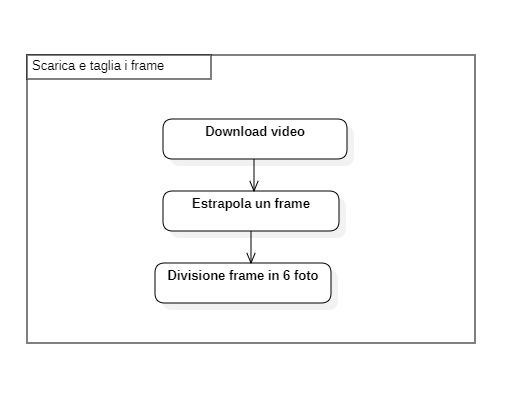
\includegraphics[scale=0.8]
    {../immagini/diag_PB/download_e_cut_frames.png}
		\caption{Diagramma di sotto attività di scarica e taglia i frame}
	\end{figure}
\end{center}

\subsubsection{Diagramma di sotto attività di riconoscimento persone}\label{DiagrammaSottoAttivitaRiconoscimentoPersone}
\begin{center}
	\begin{figure}[H]
		\centering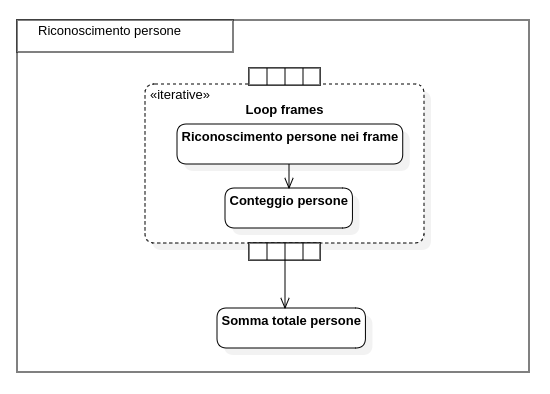
\includegraphics[scale=0.8]
    {../immagini/diag_PB/conta_persone.png}
		\caption{Diagramma di sotto attività di riconoscimento persone}
	\end{figure}
\end{center}

\subsubsection{Diagramma di attività di Kafka}\label{DiagrammaDiKafka}
\begin{center}
	\begin{figure}[H]
		\centering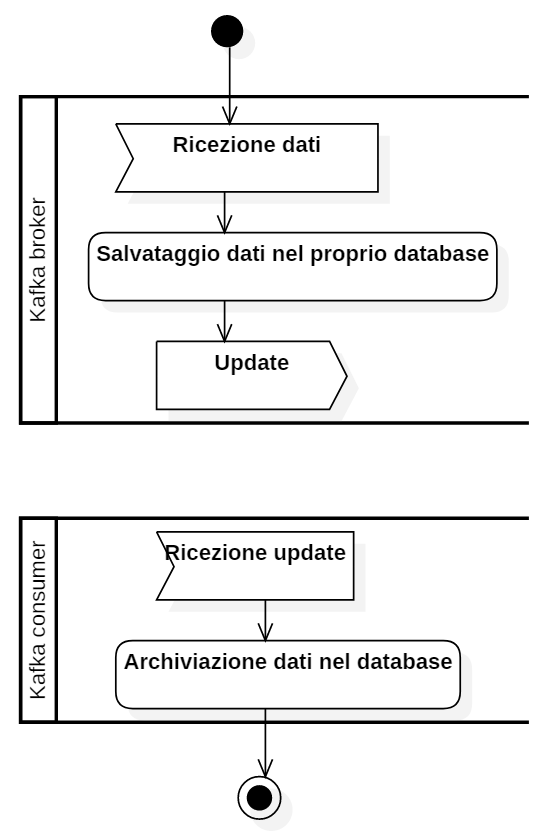
\includegraphics[scale=0.8]
    {../immagini/diag_PB/kafka.png}
		\caption{Diagramma di attività Kafka}
	\end{figure}
\end{center}


\section{Architettura della predizione}\label{ArchitetturaDelProdottoPrediction}
L'architettura del modulo del machine-learning$_{\scaleto{G}{3pt}}$ si può semplificare ad un modulo unico con all'interno i metodi necessari per prelevare dati dal database per generare delle predizioni ed archiviarle nel database.
Non necessita classi interne in quanto svolge esclusivamente operazioni procedurali. 
%Inserire
%Grafici
\subsection{Diagrammi dei package}\label{DiagrammaDeiPackagePrediction}
\begin{center}
	\begin{figure}[H]
		\centering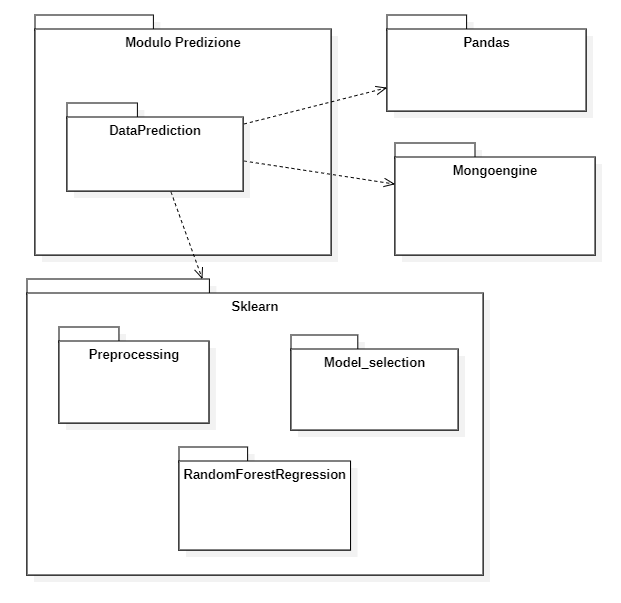
\includegraphics[scale=0.8]{../immagini/diag_PB/diag_pack_pred.png}
		\caption{Diagramma dei package del modulo predizione}
	\end{figure}
\end{center}

\subsection{Diagrammi di attività}\label{DiagrammaDiAttivitaPrediction}
\begin{center}
	\begin{figure}[H]
		\centering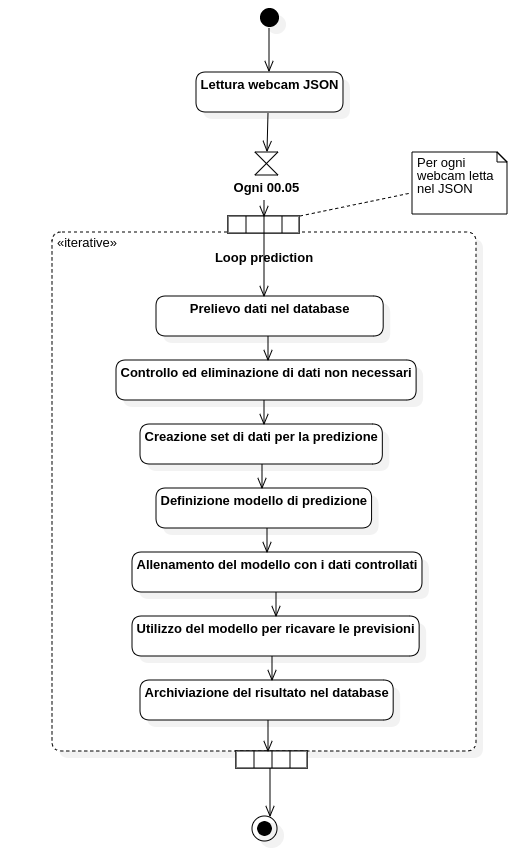
\includegraphics[scale=0.60]{../immagini/diag_PB/prediction_activity.png}
		\caption{Diagramma di attività del modulo predizione}
	\end{figure}
\end{center}


\section{Architettura Web-App}\label{ArchitetturaDelProdottoWebApp}
Lo scambio di dati tra fron-end$_{\scaleto{G}{3pt}}$ e back-end$_{\scaleto{G}{3pt}}$ avviene attraverso il design pattern$_G$ architetturale REST$_{\scaleto{G}{3pt}}$. Si ha optato per questo pattern in modo da avere un oggetto unico strutturalmente di scambio tra le due parti e quindi non vincolato  dalla  struttura  presente  nel  database.
Questo permette di aumentare la portabilità dell'applicazione web potendo applicare il back-end$_{\scaleto{G}{3pt}}$, possibilmente, a diversi front-end$_{\scaleto{G}{3pt}}$. Le richieste che il front-end$_{\scaleto{G}{3pt}}$ effettua al back-end$_{\scaleto{G}{3pt}}$ sono HTTP Request GET, quindi sono sempre richieste di visione di informazioni per poi essere utilizzate per aggiornare la parte grafica visibile dal client.
%Inserire
%Grafici
\subsection{Diagrammi dei package del modulo back-end}\label{DiagrammaDeiPackageRestApi}
Il diagramma dei package del modulo back-end$_{\scaleto{G}{3pt}}$ espone le classi all'interno del modulo e l'uso della libreria esterna framework di Spring per generare il servizio REST$_{\scaleto{G}{3pt}}$ con l'autoconfigurazione messa a disposizione da Spring Boot.
\begin{center}
	\begin{figure}[H]
		\centering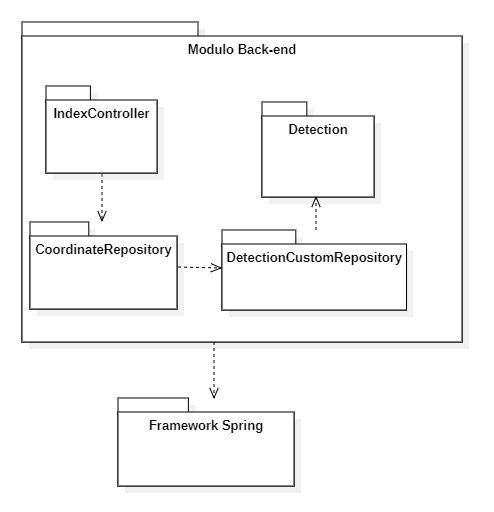
\includegraphics[scale=0.8]{../immagini/diag_PB/diag_pack_spring.png}
		\caption{Diagramma dei package del modulo back-end}
	\end{figure}
\end{center}
\subsection{Diagramma delle classi del modulo back-end}\label{DiagrammaClassiRestApi}
\begin{center}
	\begin{figure}[H]
		\centering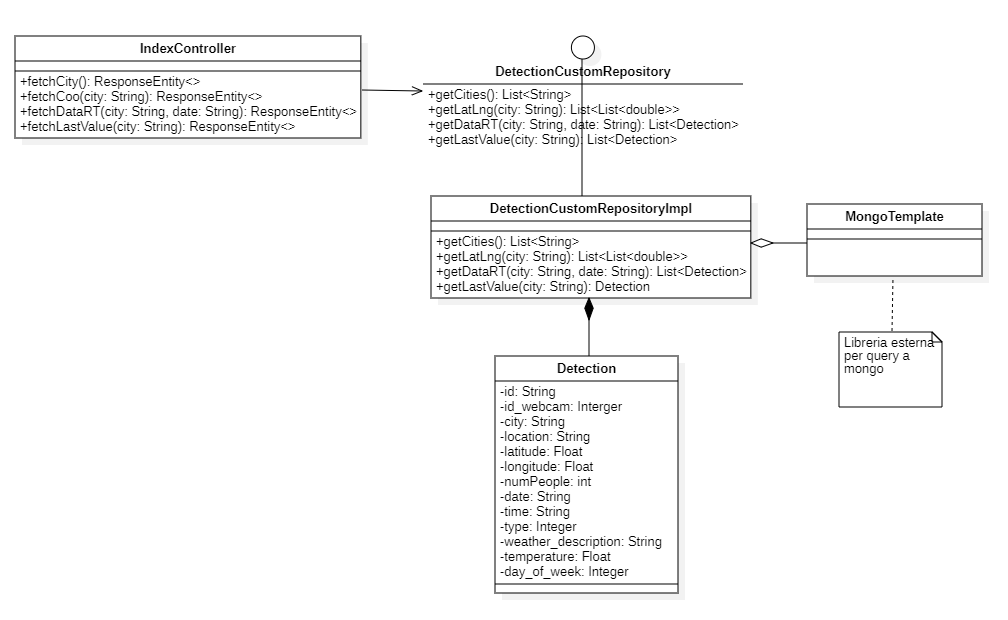
\includegraphics[scale=0.65]{../immagini/diag_PB/diag_class_spring.png}
		\caption{Diagramma delle classi del modulo back-end}
	\end{figure}
\end{center}
\subsection{Diagramma di sequenza del modulo back-end}\label{DiagrammaSequenzaSpring}
Il diagramma di sequenza illustrato descrive la sequenza di azioni dopo una richiesta di visualizzazione della lista delle città presenti nel database. Questo schema omette tutte le componenti create autonomamente da Spring Boot$_{\scaleto{G}{3pt}}$. Tutte le altre richieste hanno uno schema analogo, ma con una query diversa al database.
\begin{center}
	\begin{figure}[H]
		\centering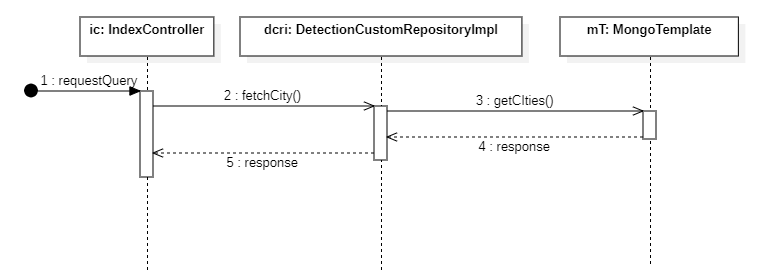
\includegraphics[scale=0.7]{../immagini/diag_PB/diag_seq_spring.png}
		\caption{Diagramma di sequenza del modulo back-end}
	\end{figure}
\end{center}
\subsection{Diagrammi dei package del modulo front-end}\label{DiagrammaPackageFrontEnd}
Il diagramma dei package del modulo front-end$_{\scaleto{G}{3pt}}$ espone i collegamenti tra i vari file e componenti dell'applicazione sviluppata in Vue$_{\scaleto{G}{3pt}}$.
\begin{center}
	\begin{figure}[H]
		\centering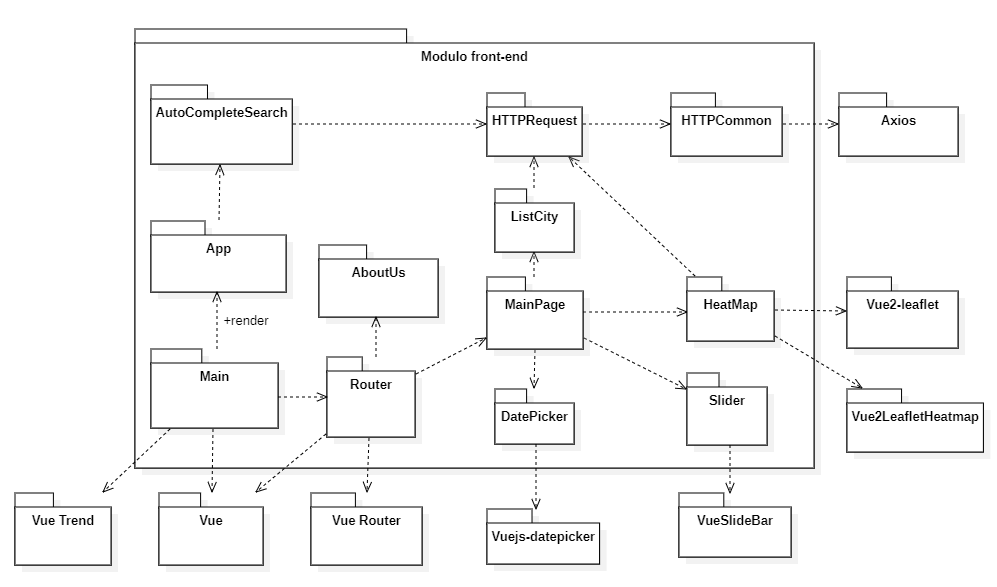
\includegraphics[scale=0.7]{../immagini/diag_PB/diag_pack_vue.png}
		\caption{Diagramma dei package del modulo front-end}
	\end{figure}
\end{center}
\subsection{Diagrammi delle attività}\label{DiagrammaDelleAttivita}
In questo diagramma di attività viene illustrata la sequenza di operazioni dell'aggiornamento della heat-map a seguito di un cambiamento dei parametri della web-app da parte dell'utente.
\begin{center}
	\begin{figure}[H]
		\centering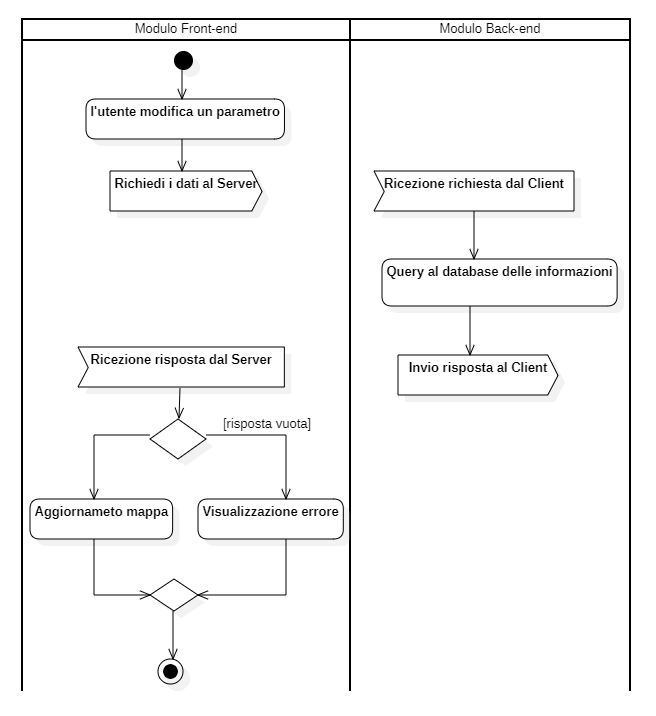
\includegraphics[scale=0.8]{../immagini/diag_PB/diag_act_front_back.png}
		\caption{Diagramma di attività tra modulo front-end e modulo back-end}
	\end{figure}
\end{center}
